\documentclass[fleqn,10pt,lineno]{olplainarticle}
% Use option lineno for line numbers

\graphicspath{{../figures/}}

\usepackage[implicit=false]{hyperref}
\usepackage{acronym}

\title{Assessing United States county-level exposure for research on tropical cyclones and human health}

\author[a,1]{G. Brooke Anderson} 
\author[a,b]{Joshua Ferreri}
\author[c]{Mohammad Al-Hamdan} 
\author[c]{William Crosson} 
\author[d]{Andrea Schumacher} 
\author[e]{Seth Guikema} 
\author[f]{Steven Quiring} 
\author[g]{Dirk Eddelbuettel} 
\author[a]{Meilin Yan} 
\author[h]{Roger D. Peng}

\affil[a]{Department of Environmental \& Radiological Health Sciences, Colorado 
  State University, Fort Collins, CO, 80523} 
\affil[b]{University of Colorado Denver School of Medicine, Aurora, CO, 80045} 
\affil[c]{Universities Space Research Association, NASA Marshall Space Flight 
  Center, Huntsville, AL, 35805}
\affil[d]{Cooperative Institute for Research in the Atmosphere, Colorado State
  University, Fort Collins, CO, 80523} 
\affil[e]{Department of Industrial and Operations Engineering, University of 
  Michigan, Ann Arbor, MI, 48109}
\affil[f]{Department of Geography, Ohio State University, Columbus, OH, 43210}
\affil[g]{Debian and R Projects; Department of Statistics, University of
  Illinois at Urbana-Champaign, Champaign, IL, 61820} 
\affil[h]{Department of Biostatistics, Johns Hopkins Bloomberg School of Public 
  Health, Baltimore, MD, 21205}

\keywords{Hurricanes, Tropical cyclones, Disaster impacts, Exposure assessment}

\begin{abstract} 
  \begin{abstract}

\noindent \textbf{Background:} 
        Tropical cyclone epidemiology can be 
	advanced through county-level exposure assessment methods that are comprehensive and 
	consistent across space and time, allowing multi-year, multi-storm studies. 
	Further, an understanding of 
	patterns in and between hazard-specific exposure metrics can help in 
	designing tropical cyclone epidemiological studies.\\ 
\textbf{Objectives:} (1)~Provide an open-source dataset for tropical
	cyclone exposure assessment for epidemiological research and
	(2)~investigate patterns and agreement between county-level assessments of tropical cyclone
	exposure based on different storm hazards. \\ 
\textbf{Methods:} We created an open-source dataset with county-level data on
	exposure to four tropical cyclone hazards: maximum sustained winds,
	rainfall, flooding, and tornadoes. The data cover all eastern \ac{US} counties 
	for all land-falling or near-land
	Atlantic basin storms for~1996\,--\,2011 for all
	metrics and up to~1988\,--\,2015 for specific metrics. 	
	We validated 
	measurements against other data sources and investigated patterns
	and agreement among binary exposure classifications based on these
	metrics, as well as between distance from the storm's track as a proxy for
	exposure.\\ 
\textbf{Results:} Measurements in the dataset created here typically
        agreed with data from other sources, and we present and discuss areas of
	disagreement and other caveats for the data.
        Long-term geographic patterns in exposure classification agree with previous results from
	atmospheric science. County-level exposure classification for a storm differs substantially 
	depending on the hazard metric used. \\ 
\textbf{Discussion:} Our results provide a multi-hazard dataset that can be
	leveraged for epidemiologic research on tropical cyclones, as well as 
	insights that can inform the design of tropical cyclone epidemiological 
	studies.
\end{abstract}

\end{abstract}

\begin{document}

\flushbottom 
\maketitle 
\thispagestyle{empty}

\section*{Introduction}

\acresetall

Recently, several major tropical cyclones have hit \ac{US} cities, including
Hurricanes Harvey, Irma, and Maria in 2017 \parencite{blake20182017} and
Hurricanes Florence and Michael in 2018 \parencite{avila20192018}. Researchers
are exploring how these storms impacted human health (e.g.,
\parencite{santos2018use, rivera2018estimating, santos2018differential,
grineski2019impact, issa2018deaths, tanz2019notes, paul2019brief}), including
through projects funded through \ac{NIH} Rapid Response grants
\parencite{nihreporter}. These projects will add to evidence from previous
hurricanes, including Sandy in 2012 (e.g., \parencite{swerdel2014}) and Katrina
in 2005 (e.g., \parencite{burton2009health}), characterizing the health impacts
of hurricanes. 

A recent review highlights the need to supplement these single-storm studies
with multi-year, multi-storm studies, to identify patterns that are common
across multiple storms [ref]. While multi-year studies of hurriance mortality
impacts have been conducted using disaster surveillance data, studies based on
administrative data could identify risks for non-accidental mortality and
morbidity that those studies likely undercount [ref]. Multi-storm studies with
administrative data require exposure assessment that is consistent across time
and space, allowing the administrative data to be linked to disaster exposure
[ref]. Key to expanding tropical cyclone epidemiology are therefore exposure
assessment methods that appropriately capture hazards of the storm that are
relevant to human health, methods that can be applied consistently across
multiple storms, locations, and years. 

The \ac{NHC} publishes a ``Best Tracks'' dataset that is considered the gold
standard for Atlantic-basin tropical cyclone tracks.  It records the central
position of a tropical cyclone every six hours, as well as the storm's
\underline{minimum pressure} and \underline{central maximum sustained winds}. This data is openly
available through the \ac{HURDAT2}, a post-storm assessment conducted
by the \ac{US} \ac{NHC} that incorporates data from a variety of sources,
including satellite data and, when available, aircraft reconnaissance
data~\parencite{landsea2013, jarvinen1988}. With this data, it is
straightforward to measure whether a community was in the direct path, or
within a certain distance of the path, of a storm. Some studies have indeed
used this data to assess tropical cyclone exposure based on how near the
storm's central track came to the county, either to assess average exposure
patterns to tropical storms [refs] or to characterize exposure for health
studies [refs].

When epidemiological studies assess exposure to a tropical cyclone based on 
how close the storm came to a community, however, they may misclassify exposure. 
Tropical cyclones vary dramatically in size: \ac{US} tropical
cyclones have been observed with radii to maximum winds as small
as~20~\si{\kilo\metre} and as large
as~200~\si{\kilo\metre}~\parencite{mallin2006, quiring2011variations}.  While a
number of tropical cyclone hazards are strongly associated with distance from
the tropical cyclone's center (e.g., wind and, at the coast, storm surge and
waves~\parencite{rappaport2000, kruk2010}), other hazards like heavy rainfall,
floods, and tornadoes can occur well away from the tropical cyclone's central
track~\parencite{rappaport2000, atallah2007, moore2012}.  For example, fatal
tropical cyclone tornadoes, which were linked to over~300 deaths in the \ac{US}
between~1995 and~2009, most often occur~200\,--\,500~\si{\kilo\metre} from the
tropical cyclone's center~\parencite{moore2012}.  

Further, when studies use distance from the storm's track to assess exposure,
they often use an equal buffer distance on each side of the tropical cyclone
track (e.g.,~\cite{czajkowski2011, grabich2015, grabich2016, zandbergen2009,
tansel2010}). However, the forces of a tropical cyclone tend to be distributed
around the center in a non-symmetrical way. Extreme winds are more common to
the right of the track, where counter-clockwise cyclonic winds move in concert
with the tropical cyclone's forward motion~\parencite{halverson2015}, and the
fatal tornadoes associated with \ac{US} tropical cyclones between~1995 and~2009
occurred almost exclusively to the right of the tropical cyclone's track,
mostly in the right front quadrant of the tropical
cyclone~\parencite{moore2012}. Rain, conversely, is often heaviest to the left
of the tropical cyclone's track, especially when the tropical cyclone interacts
with other weather systems~\parencite{atallah2003, atallah2007,
zhu2013variations} or undergoes an extratropical
transition~\parencite{elsberry2002}.

If a study misclassifies exposure to the hazard or hazards that cause the
health risk being studied, the study will generate biased estimates of tropical
cyclone risks and impacts. Further, when different studies use different
methods to assess exposure to tropical cyclones, their results are difficult to
meaningfully compare and aggregate. If different methods identify
similar sets of communities as ``exposed'',  these concerns are less serious.
However, if different methods differ substantially in which communities they
identify as ``exposed'', it makes it very important that epidemiological
studies are thoughtful in how they assess exposure.

To provide open-source data on tropical cyclone exposures to other researchers,
we developed a dataset of county-level exposure to tropical cyclones in all
eastern \ac{US} counties for five different metrics
(Table~\ref{tab:exposuremetrics}): (1)~distance to tropical cyclone track;
(2)~maximum sustained wind speed; (3)~cumulative rainfall; (4)~flood events;
and (5)~tornado events~\parencite{hurricaneexposure}. This data is provided at
the county level since data on many potential impacts are available at
county-level aggregations (e.g., direct hurricane-related
deaths~\parencite{czajkowski2011}; birth outcomes~\parencite{grabich2015,
grabich2016}; autism prevalence~\parencite{kinney2008}) and since decisions and
policies to prepare for, and respond to, tropical cyclones are often undertaken
at the county level~\parencite{zandbergen2009, rappaport2000}. Further, we
explored patterns in these exposure assessments across storm hazards and
measured how well exposure classification agreed across these five metrics in
terms of classifying specific counties as exposed to a tropical cyclone.  


\begin{table}%[tbhp] 
\centering 
\caption{Exposure metrics considered to assess county-level exposure to 
tropical cyclones}
\begin{tabular}{p{0.9cm}p{2.5cm}p{9cm}} 
Metric & Available & Criteria for exposure \\ \midrule 
Distance & 1988--2015 & County population mean center within 100 kilometers of storm track \\ 
Rain & 1988--2011 & County cumulative rainfall of 75 millimeters or more over the period from two days before to one day after the storm's closest approach and county population mean center within 500 kilometers of the storm track \\ 
Wind & 1988--2015 & Modeled maximum sustained wind speed at the county's population mean center 15 meters per second or higher during the storm\\ 
Flood & 1996--2015 & Flood event listed in the National Oceanic and Atmospheric Administration (NOAA) Storm Events database for the county with a start date within two days of the storm's closest approach and county population mean center within 500 kilometers of the storm track \\
Tornado & 1996--2015 & Tornado event listed NOAA Storm Events database for the county with a start date within two days of the storm's closest approach and county population mean center within 500 kilometers of the storm track\\
\bottomrule 
\end{tabular} 
\label{tab:exposuremetrics} 
\end{table}

\section*{Methods and Materials}

This study covered all counties in the eastern half of the \ac{US}
(Figure~\ref{fig:hurrtracks}), as of the~2010 \ac{US} Decennial Census. The
study covered all tracked land-falling or near-land Atlantic-basin tropical
cyclones between~1988 and~2015, considering all 136 storms in \ac{HURDAT2}
\parencite{landsea2013} that came within~250 \si{\kilo\metre} of at least one
eastern \ac{US} county in this period (Figure~\ref{fig:hurrtracks}). 

\begin{comment}
These data typically give measurements of
the tropical cyclone center's location [and central pressure / maximum
windspeed?] at~6-\si{\hour} intervals at synoptic times (i.e., 6:00~am,
12:00~pm, 6:00~pm, and 12:00~am \ac{UTC}); some landfalling tropical cyclones
have an additional observation at the time of landfall~\parencite{landsea2013}.
\end{comment}

\subsection*{Distance-based exposure metric}

We first measured how close each study storm came to each study county. We
started with tracking data from \ac{HURDAT2}, which records the storm's
position every~6 \si{\hour}, and interpolated to~15-\si{\minute} intervals
using natural cubic splines~\parencite{hurricaneexposure}. We then measured the
distance between the storm's position at each~15-\si{\minute} interval and each
county's population mean center, as assessed by the 2010 Decennial
Census~\parencite{countycenters}, using the Great Circle (WGS84 ellipsoid)
method~\parencite{bivand2013applied}. These measurements captured the distance
between the storm's central track and each study county throughout the period
when the storm was tracked. The closest distance between the storm and each
county was recorded as the distance of the storm's closest approach to the
county. We also recorded the time storm came closest to each county, for use in
assessing rain-, flood-, and tornado-based metrics where observed data on the
hazards needed to be matched by time to storm events.  To allow matching with
data based on local time, times were converted from \ac{UTC} to local
time~\parencite{countytimezones}.

\subsection*{Rain-based exposure metric}

To estimate storm-associated rainfall, we used precipitation data from a
re-analysis dataset, as this data was available for every county and every day
through a continuous period of the study
(1988\,--\,2011)~\parencite{alhamdan2014environmental, cdcwonder}.  By
comparison, observations from ground-based monitoring networks had missing
values spatially (i.e., for some study counties), temporally (for some days),
or both.  

We estimated daily rainfall for each study county by aggregating
hourly~1/8\si{\degree} gridded reanalysis data from the \ac{NLDAS-2}
precipitation data files~\parencite{rui2013nldas}. These data integrate
satellite-based and land-based monitoring, applying a land-surface model to
create a reanalysis dataset that is spatially and temporally complete across
the continental \ac{US}~\parencite{rui2013nldas, alhamdan2014environmental}. To
aggregate to county-level, the hourly data at each grid point were summed to
create a daily rainfall total, and these grid point rainfall totals were then
averaged across all grid points within a county's~1990 \ac{US} Census
boundaries~\parencite{alhamdan2014environmental, cdcwonder}. These daily
county-level estimates were then matched temporally with storm tracks, using
the date when each storm was closest to each county. The cumulative
storm-associated rainfall was then calculated as the sum of rainfall from two
days before the storm's closest approach to a county to one day after, as 
storm-related rains often precede the passing of the storm's center. 

To validate these rainfall estimates, we investigated a subset of counties that
also had available ground-based precipitation observations. We selected nine
sample counties geographically spread across storm-prone regions of the eastern
\ac{US} and for which precipitation data were available from multiple stations
throughout the study period: Miami-Dade, FL; Harris County, TX; Mobile County,
AL; Orleans Parish, LA; Fulton County, GA; Charleston County, SC; Wake County,
NC; Baltimore County, MD; and Philadelphia County, PA. We collected
ground-based observations of precipitation data from all stations in the county
with available daily data in the Global Historical Climatology Network
throughout 1988\,--\,2011~\parencite{menne2012overview, rnoaa, countyweather}.
We summed daily station-specific measurments for two days before to one day
after each storm's closest approach and then averaged these cumulative
station-based precipitation totals for each county as a county-wide estimate of
cumulative storm-related precipitation. We measured the rank correlation
(Spearman's~$\rho$~\parencite{spearman1904proof}) between storm-specific
cumulative precipitation estimates for the two data sources within each sample
county.

\subsection*{Wind-based exposure metric}

Ground-based observations of wind speed are problematic as a metric of exposure
to tropical cyclones, as instruments often fail at high wind speed, while
reanalysis data, often available at hourly or higher resolution, can lack a
fine enough temporal resolution to capture wind extremes associated with a
tropical cyclone. Therefore, to create a dataset of county-level sustained
winds during historical tropical cyclones, we modeled maximum sustained wind
speeds at each county's population mean center~\parencite{countycenters}, using
a wind speed model based on results from
Willoughby~\parencite{willoughby2006parametric}. For each storm, we used the
interpolated storm tracks generated for the distance metric and, for
each~15-\si{\minute} increment, we modeled maximum ground-level sustained wind
speed at each county center using a double exponential wind speed model with
inputs for the storm's forward speed, direction, and central wind
speed~\parencite{willoughby2006parametric, stormwindmodel}. This model
incorporated asymmetry in wind speeds around the tropical cyclone center that
results from the storm's forward movement~\parencite{phadke2003modeling,
stormwindmodel}. We then determined the maximum value of this estimate over the
storm tracking period for each study county to determine the maximum sustained
surface wind speed in each county during each storm.

To validate these modeled county-level wind speed estimates, we compared them
to county-level maximum sustained surface wind speeds based on the wind radii
estimates in \ac{HURDAT2}, which are based on \ldots. The wind radii values
have been included in \ac{HURDAT2} since 2004 [?] and estimate the distance
from the storm's center to the furthest point with winds at or above winds of a
certain speed in each four quadrants of the storm. They give estimates of these
maximum radii for three thresholds of maximum surface wind speeds: 64,~50,
and~34 \si{\knot}.  They therefore allow for the classification of counties
into four categories of maximum sustained wind speeds: $<$34~\si{\knot};
34\,--\,49.9~\si{\knot}; 50\,--\,63.9~\si{\knot}; $\ge$64~\si{\knot}. We
interpolated this data to~15-\si{\minute} increments and classified a county as
exposed to winds in a given wind speed category if its population mean center
was within~85\% of the maximum radius for that wind speed in its quadrant of
the storm [clarify why 85\%]. We compared these wind radii-based estimates with
the modeled wind speed estimates for the study storms since 2004 for which at
least one study county had a sustained wind of~$\ge$34 \si{\knot} (based on the
\ac{HURDAT2} wind radii). For each of these storms, we calculated the percent
of study counties that were classified in the same wind speed category.

\subsection*{Flood- and tornado-based exposure metrics}

To identify flood- and tornado-based tropical cyclone exposures in \ac{US}
counties, we used event listings from the National Oceanic and Atmospheric
Administration (NOAA)'s Storm Event Database~\parencite{stormevents}. For each
tropical cyclone, we identified all events with event types related to flooding
(``Flood", ``Flash Flood", ``Coastal Flood") and tornadoes (``Tornado") and
that occurred in a county within~500 \si{\kilo\metre} of the tropical cyclone's
track and with a start date within a five-day window centered on the date of
the tropical cyclone's closest approach to the
county~\parencite{hurricaneexposuredata}. ``Flood", ``Flash Flood" and
``Tornado" events in this database were reported by county \ac{FIPS} code and
so could be directly linked to counties.  ``Coastal Flood" events were reported
by forecast zone; for these, the event was matched to the appropriate county if
possible using regular expression matching of listed county
names~\parencite{noaastormevents}. While this database has recorded storm data
since~1950, its coverage changed substantially in~1996 to cover a wider variety
of storm events~\parencite{stormevents}. We therefore only considered these
metrics of hurricane exposure for tropical cyclones in~1996 and later.

The tornado observations from this dataset form the traditional tornado event
database for the \ac{US}, and so we did not conduct analyses to validate the
tornado event data. It is difficult to characterize flooding at the county
level because flooding can be very localized and can be triggered by a variety
of causes. To investigate the extent to which the NOAA flood event data
captures extremes that might be identified with other flooding data sources, we
investigated a sample of study counties, comparing the flood event data during
tropical storms with streamflow measurements at \ac{US} Geological Survey
county streamflow gages \parencite{usgsgages, countyfloods, dataRetrieval}.  

We considered nine study counties, selecting counties geographically spread
through storm-prone areas of the eastern \ac{US} and with multiple streamflow
gages reporting data during events (Baltimore County, MD; Bergen County, NJ;
Escambia County, FL; Fairfield County, CT; Fulton County, GA; Harris County,
TX; Mobile County, AL; Montgomery County, PL; and Wake County, NC). For each
county, we first identified all streamflow gages in the county that had
complete data for Jan.~1~1996\,--\,Dec.~31,~2015. If a storm did not come
within~500~\si{\kilo\metre} of a county, it was excluded from this analysis,
but all other study storms were considered. For each storm and county, we
summed daily total streamflow across all streamgages for each day in the
five-day window around the storm's closest approach. We took the maximum daily
streamflow total during those five days as a measure of the county's maximum
streamflow during that storm. We also calculated the percent of streamflow
gages in the county with a daily streamflow that exceeded a threshold of
flooding (the streamgage's median value for annual peak
flow~\parencite{countyfloods}) on any day during the five-day window. We
investigate how these measurements varied between storms with associated flood
events in the NOAA Storm Events data versus storms without an event listing, to
explore if storms with flood event listings tended to be  associated with
higher streamflows at gages within the county.

\subsection*{Binary storm exposure classifications based on different metrics}

In our open-source dataset, we provide the closest distance of each storm to
each county, as well as county-level storm-related winds and rainfall, as
continuous metrics. However, epidemiologic studies of tropical cyclones often
compare ``exposed'' versus ``unexposed'' communities to assess storm-related
health risks [refs], and so we also used these continuous metrics to classify
counties as ``exposed'' or ``unexposed'' and explored patterns in storm
exposure based on these binary clasifications. 

Two of the exposure metrics (flood- and tornado-based) were inherently binary,
since these metrics were based on whether an event was listed in the NOAA Storm
Events database.  For the other exposure metrics, each county was classified as
exposed to a tropical cyclone based on whether the exposure metric exceeded a
certain threshold (Table~\ref{tab:exposuremetrics}). For the rainfall metric, a
distance constraint was also necessary, to ensure that rains unrelated and far
from the storm track were not misattributed to a storm. Through exploratory
analysis, we set this distance metric at~500 \si{\kilo\metre} (i.e., for a
county to be classified as exposed based on rainfall, the cumulative rainfall
had to be over 75 \si{\milli\metre} and the storm must have passed within~500
\si{\kilo\metre} of the county; Table~\ref{tab:exposuremetrics}). We set this
distance constraint at a value that was typically large enough to capture
storm-related rain. However, data users should note that in rare examples of
exceptionally large storms (e.g., Hurricane Ike in 2008) or storms for which
storm tracking was stopped at extratropical transition (e.g., Tropical Storm
Lee in 2011), some storm-related rains may be missed because of this distance
constraint (Figure~S1). 

We assessed patterns in county-level tropical cyclone exposure in the eastern
\ac{US} based on each exposure metric. Depending on available exposure data,
this assessment included some or all of the period from~1988 to~2015 (Table 1).
For each binary metric of tropical cyclone exposure (Table 1), we first summed
the total number of county-level exposures over available years for each
exposure metric and mapped patterns in these exposures. We next investigated
agreement between storm exposure classifications based on different exposure
metrics. We calculated the within-storm Jaccard
index~\parencite{jaccard1901distribution, jaccard1908nouvelles} between each
pair of exposure metrics. The Jaccard index~($J_s$) measures similarity between
two metrics ($X_{1,s}$ and~$X_{2,s}$) for tropical cyclone~$s$ as the
proportion of counties in which both of the metrics classify the county as
exposed out of all counties classified as exposed by at least one of the
metrics:

\begin{equation} 
J_s = \frac{X_{1,s} \cap X_{2,s}}{X_{1,s} \cup X_{2,s}}
\end{equation}

\noindent This metric can range from~0, in the case of no overlap between the
counties classified as exposed based on the two metrics, to~1, in the case that
the two metrics classify exactly the same set of counties as exposed to the
tropical cyclone. We measured these values for all study storms that affected a
large number of eastern \ac{US} counties (250 or more of the study counties
classified as exposed by at least one of the exposure metrics) during the years
when all exposure data were available (1996\,--\,2011).

\subsection*{Case study: Physical exposure of electricity-dependent Medicare
beneficiaries to tropical cyclones}

Disasters' societal impacts depend both on the geophysical forces of the
disaster and on the vulnerability of those living in the affected geographical
areas~\parencite{chakraborty2005population, anderson2003community,
cutter1996vulnerability}. As a case study, we explored how differences in
tropical cyclone exposure assessments across different exposure metrics might
influence estimates of physical exposures of a susceptible population to
tropical cyclones. We calculated expected average physical exposures among
electricity-dependent Medicare beneficiaries in eastern \ac{US} counties to
tropical cyclones based on each exposure metric. This subpopulation was
selected since it may be particularly susceptible to health impacts from
tropical cyclone exposure, especially through the pathway of storm-associated
power outages and evacuations. 

We collected data on the number of electricity-dependent Medicare beneficiaries
in each study county from the \ac{US} Department of Health \& Human Service's
emPower Map~2.0~\parencite{empower}. We then calculated the physical exposure
of the electricity-dependent Medicare population in each county, based on
tropical cyclone assessments using each hazard metric,
following~\parencite{peduzzi2009assessing}:

\begin{equation}
E_c = F_c * P_c
\end{equation}

\noindent where~$E_c$ is the average yearly physical exposure among
electricity-dependent Medicare beneficiaries in county~$c$ to tropical cyclone
exposures based on a given metric,~$F_c$ is the estimated yearly expected
frequency of tropical cyclone exposures in county~$c$ based on that metric,
and~$P_c$ is the electricity-dependent Medicare population in
county~$c$, as of July~2017. 

\begin{comment}
When combined with estimates of vulnerability of a
population to a natural hazard, such measurements of physical exposure can be
used to calculate risk of human losses from the
hazard~\parencite{peduzzi2009assessing}.
\end{comment}




\begin{figure*}%[tbhp] 
\centering 
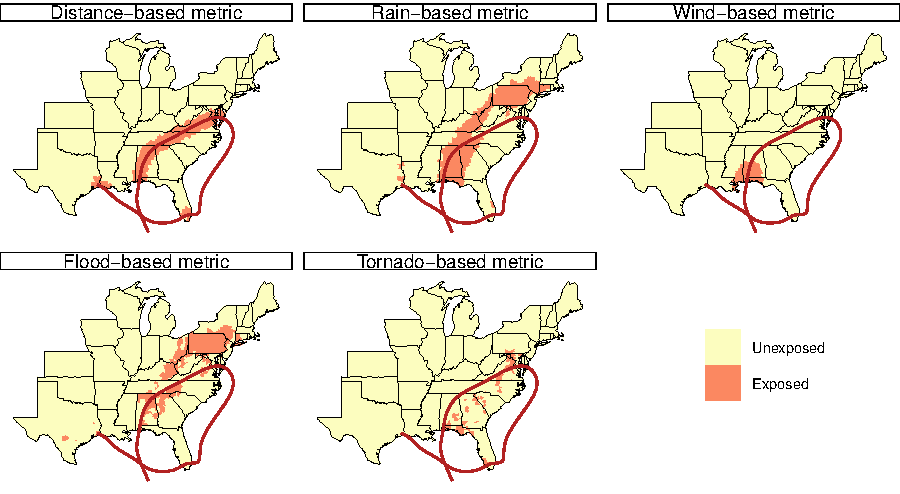
\includegraphics[width=16cm]{ivanonly}
\caption{Counties classified as exposed to Hurricane Ivan (2004) under each
exposure metric (Table 1). The red line shows the track of Hurricane Ivan 
based on the revised Atlantic hurricane database (HURDAT2 \citep{landsea2013}).
Similar maps for other large-extent storms are given in Fig. S5.}
\label{fig:ivanexposure} 
\end{figure*}

% latex table generated in R 3.4.3 by xtable 1.8-2 package
% Wed Oct 10 12:11:35 2018
\begin{table}[ht]
\centering
\caption{Summary statistics for the number of county tropical cyclone exposures under each metric.     
	 The median and interquartile range of number of county exposures per tropical cyclone are based on
         the tropical cyclones for which at least one US county was exposed. The years for which
         data are available for each metric are given in Table 1.} 
\label{tab:exposuresummaries}
\begin{tabular}{p{1.75cm}p{3cm}p{4cm}p{4cm}}
  \toprule
Metric & Mean (interquartile range) of county exposures per year & Median (interquartile range) of county exposures per tropical cyclone & Tropical cyclone with most counties exposures (\# exposed counties) \\ 
  \midrule
Distance & 433 (224, 503) & 84 (23, 173) & Beryl, 1994 (330) \\ 
  Rain & 401 (152, 553) & 68 (14, 146) & Frances, 2004 (464) \\ 
  Wind & 224 (83, 353) & 34 (8, 80) & Ike, 2008 (355) \\ 
  Flood & 213 (84, 249) & 26 (6, 57) & Ivan, 2004 (317) \\ 
  Tornado & 53 (16, 43) & 7 (2, 16) & Ivan, 2004 (91) \\ 
   \bottomrule
\end{tabular}
\end{table}


\begin{figure}%[tbhp] 
\centering 
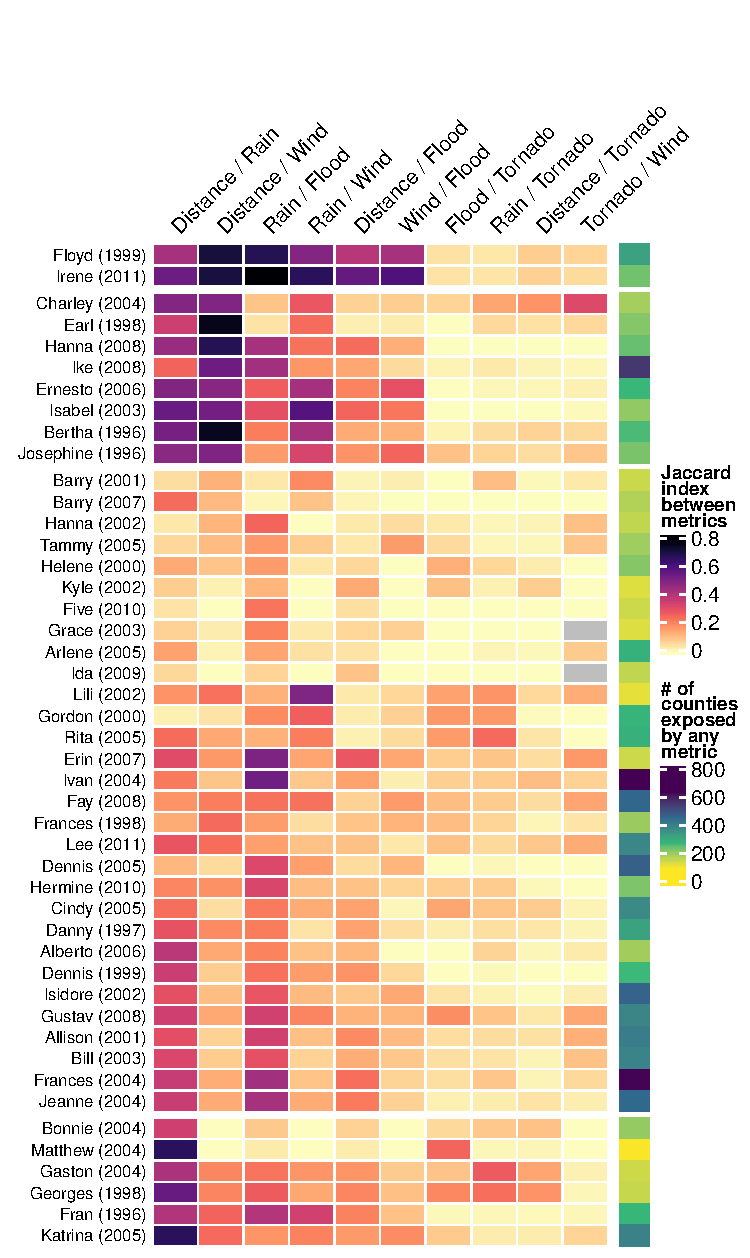
\includegraphics[width = 0.7\linewidth]{jaccard_heatmap} 
\caption{Heatmap of Jaccard index values for
specific exposure metric pairs within storms. Only storms between 1996 and 2011,
and for which at least 250 counties were exposed based on at least one metric,
are included. The color of each cell within the main heatmap indicates the value
of the Jaccard index (proportion of counties classified as exposed by both
metrics out of storms classified as exposed by either metric) for a given pair
of metrics for a given storm. Storms are displayed within clusters that have
similar patterns in county-level exposure agreement for metric pairs, based on
hierarchical clustering using the complete link method
\citep{murtagh2012algorithms} (i.e., storms in the same cluster tend to have
similar patterns for the pairwise strength of agreement among metrics); columns
are also ordered based on hierarchical clustering. The colors to the right of
the main heatmap for each storm indicate the total number of counties classified
as exposed to the storm by any of the five metrics, providing an estimate of
storm extent. Maps are available showing the counties identified as exposed
under each of five metrics for the widest-extent storm in each cluster:
Hurricane Ivan (2004) (Fig. \ref{fig:ivanexposure}) and Hurricanes Floyd (1999),
Lee (2011), Cindy (2005), and Katrina (2005) (Fig. S5).} 
\label{fig:jaccard}
\end{figure}

\begin{figure*}%[tbhp] 
\centering
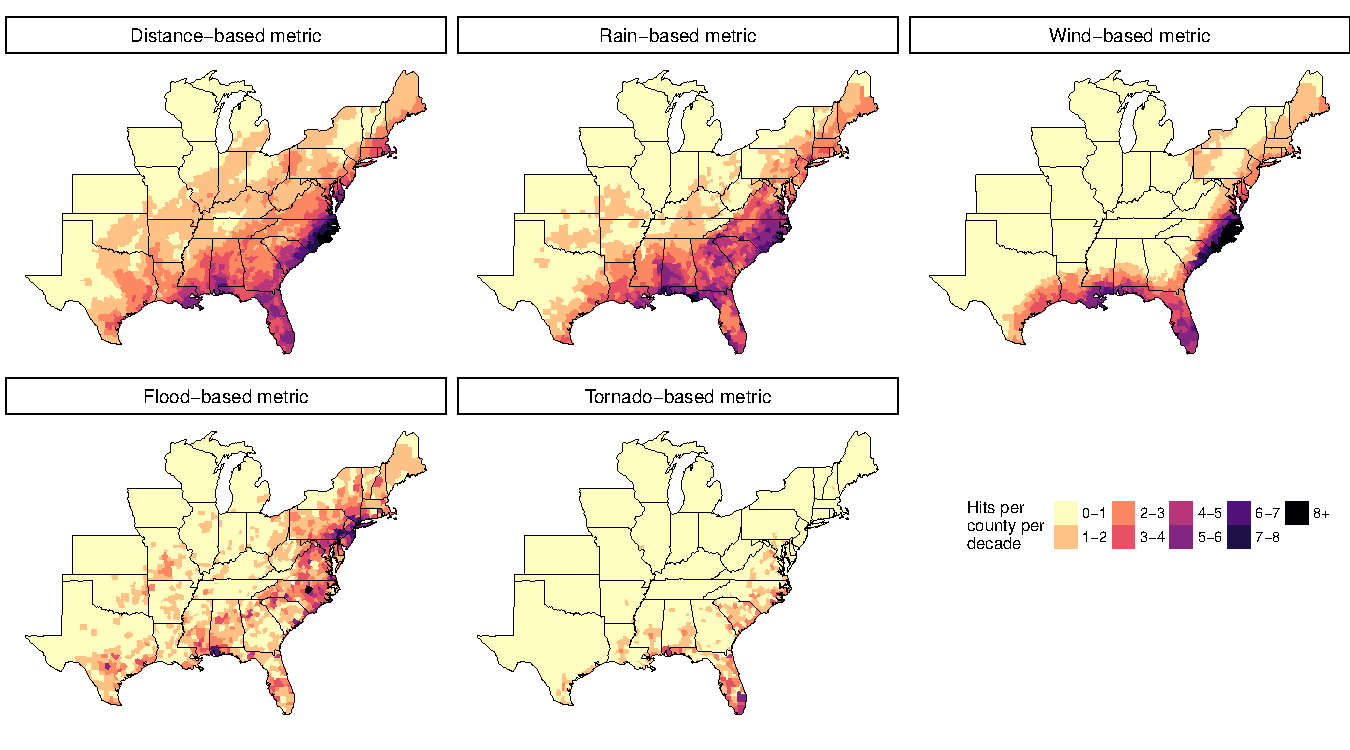
\includegraphics[width=16cm]{averageexposureonly} 
\caption{Average number of storm exposures per decade in U.S. counties for 
each exposure metric. The criteria behind each of the five metrics is given 
in Table \ref{tab:exposuremetrics}. The years used to estimate these averages 
are based on years of available exposure data (distance and wind: 1988--2015; 
rain: 1988--2011; flood and tornado: 1996--2015). Similar patterns persist when
analysis is restricted to years with all exposure data available (1996--2011;
Fig. S3).} 
\label{fig:averageexposure} 
\end{figure*}

\section*{Results}

\subsection*{Exposure assessment data, data validation, and software}

We created and published this tropical cyclone exposure data as an R
package~\parencite{hurricaneexposuredata}.  The package size exceeded the
recommended maximum size for \ac{CRAN}, the standard repository for publishing
R packages. Therefore, we used the \textit{drat} framework to set up our own
repository to host the package~\parencite{anderson2017hosting}. These data
include continuous county-level measurements for the closest distance of each
storm, cumulative rainfall, and peak sustained surface wind. These continuous
metrics can be used for classifying counties as exposed or unexposed---using
thresholds selected by the user---or can be extracted directly as continuous
metrics. The dataset also includes binary data on flood and tornado events
associated with each storm in each county. To accompany these data, we
published an additional R package with software tools to explore and map the
data and to integrate it with human health
datasets~\parencite{hurricaneexposure}.

We explored potential limitations in these data by comparing them with data
from other available sources.  For estimates of storm-associated rainfall, we
compared data in the open-source package with ground-based observations in nine
sample counties (Figure~\ref{fig:raincomparison}). Within these counties,
storm-related rainfall measurements were well-correlated between the two data
sources, with rank correlations (bottom right of each graph in
Figure~\ref{fig:raincomparison}) between 0.87 and 0.98.  There was some
evidence that our primary rainfall metric may tend to underestimate rainfall
totals in storms with extremely high rainfall, based on a few heavy-rainfall
storms in Harris County, TX, Mobile County, AL, Charleston County, SC, and Wake
County, NC (Figure~\ref{fig:raincomparison}). \textbf{Further, in some
counties, the correlation was substantially lower when considering only
tropical cyclones with cumulative local rainfall of $\ge75$ mm (Supplemental
Table 2).} However, it was rare for a storm to be classified differently (under
the precipitation threshold of 75~\si{\milli\metre} we used for binary exposure
classification for later analysis) based on the source of precipitation data.
Horizontal and vertical lines in each small plot in
Figure~\ref{fig:raincomparison} show the threshold of 75~\si{\milli\metre}, so
storms in the lower left and upper right quadrants would be classified the same
(``exposed'' or ``unexposed'') regardless of the precipitation data source,
while storms in the upper left and lower right quadrants would be classified
differently. Such cases were rare.

For peak sustained surface wind estimates, we found that the primary wind
exposure metric in the open-source data generally agreed well with the wind
radii reported in \ac{HURDAT2}. For most storms, $\>$90\% of counties were
assigned the same category of wind speed ($<$34~kt; 34\,--\,49.9~kt;
50\,--\,63.9~kt; $\ge$64~kt) by both data sources
(Figure~\ref{fig:windcomparison}).  Disagreement was limited to a few storms
(e.g., Hurricanes Sandy in 2012 and Ike in 2008). For these two storms, the
modeled wind speed in the open-source data somewhat overestimated the severity
of the storm's winds at landfall but then underestimated, particularly for
Hurricane Sandy, how far 34\,--\,49.9 kt winds extended from the storm's
central track further inland (Figure~S2). For epidemiology researchers who
would like to conduct sensitivity analysis using both sets of wind data,
we have included estimates from the \ac{HURDAT2} wind radii as a secondary
measure of county-level peak sustained wind in the open-source dataset
\parencite{hurricaneexposuredata}.

For flood data, we compared the flood status values included in the open-source
data to streamflow measurements at \ac{US} Geological Survey gages within nine
sample counties (Figure~\ref{fig:floodcomparison}). Across the sampled
counties, streamgage data generally indicated higher discharge during periods
identified as flood events based on the NOAA Storm Events database
(Figure~\ref{fig:floodcomparison}). There were some cases, however, where the
two flooding data sources were somewhat inconsistent.  For example, there were
one or two tropical cyclones in several of the counties (Mobile County, AL,
Escambia County, FL, Fairfield County, CT, and Fulton County, GA) with
associated flood event listings but for which the total discharge across county
streamflow gages was relatively low. For storms without a flood listing for the
county, in most cases the total streamflow discharge in the county was
relatively low, and, in all but two cases all streamgage flows were
below the flooding threshold. The exceptions were for Hurricane Ida in 2009 in
Fulton County, GA, and Hurricane Isaac in 2012 in Mobile County, AL. 

\subsection*{Patterns in tropical cyclone exposures}

We used this storm exposure data to classify counties as exposed or unexposed
to four different hazards for each tropical cyclone and then explored patterns
over years with available data. \textbf{Table~\ref{tab:exposuresummaries}
provides summary statistics describing the extent of counties assessed as
exposed based on specific storm hazards, to help epidemiologists in planning
studies, including understanding the potential statistical power to study
specific exposures, both for multi-storm and single-storm studies.} Across the
four storm hazards considered, there was wide variation in the average number
of county exposures per year. For tropical cyclone tornadoes, there were on
average about 40 county exposures per year within our study.  County exposures
were more frequent for tropical cyclone wind exposures ($>$160 / yr on
average), even more frequent for tropical cyclone flood exposures ($>$190 / yr
on average), and most frequent for tropical cyclone rain exposure ($>$290 / yr
on average). For every hazard except tornadoes, we identified at least one
tropical cyclone that exposed over~250 counties
(Table~\ref{tab:exposuresummaries}).  However, the largest-extent tropical
cyclone varied across hazards: Frances in~2004 exposed the most counties based
on rain, Michael in~2018 based on wind, and Ivan in 2004 based on flooding and
tornadoes (Table~\ref{tab:exposuresummaries}).

When we calculated and mapped the average number of exposures per decade in
each county for single-hazard exposures (Figure~\ref{fig:averageexposure}),
strong geographical patterns were clear. Peak sustained wind exposure had a
strong coastal pattern, with almost all exposures in counties within about~200
\si{\kilo\metre} (124~mi) of the coastline. While tropical cyclone rain
exposure was also more frequent in coastal areas compared to inland areas,
there were also inland rain exposures in counties that were rarely or never
classified as exposed based on wind. Flood-based exposures were frequently in
the Mid-Atlantic region, with a pattern that skewed north compared with other
exposures. Rain and, to some extent, flood exposures were characterized by a
pattern defined by the Appalachian Mountains, with fewer exposures west of the
mountain range than to the east. Almost all tornado-based exposures were in
coastal states, with many in Florida, and almost none north of Maryland.
Patterns were similar when analysis was restricted to years with exposure data
for all four hazards available (1996\,--\,2011; Figure~S3). 

\subsection*{Agreement across exposure metrics}

Finally, we assessed within-storm agreement between exposure classifications
for each pair of hazards, as well as with a proxy measurement based on distance
from the storm's track. We found that these exposure classifications typically
did not agree strongly between pairs of metrics---the set of counties
identified as ``exposed'' based on one metric often overlapped little with the
set identified as ``exposed'' by another metric, as storms frequently brought
different hazards to different locations. 

Figure~\ref{fig:ivanexposure} shows as an example Hurricane Ivan in 2004.
For the distance-based metric, the counties assessed as exposed follow the
tropical cyclone's track. For the wind-based metric,
only counties near the tropical cyclone's first landfall were assessed as
exposed. For rain- and flood-based metrics, however, exposure extended to the
left of the track, including counties as far north as New York and Connecticut,
while for the tornado metric, exposed counties tended to be to the right of the
track and included several counties in central North Carolina, South Carolina,
and Georgia that were not identified as exposed to Ivan based on any other
metric. Figure~S4 provides similar maps for three other example tropical
cyclones (selected because they exposed many \ac{US}  counties based on at
least one metric).

We drew similar conclusions when we investigated all~46 tropical cyclones
between~1996 and~2011 (when data for all five metrics were available) for
which~100 or more counties were exposed based on at least one metric
(Figure~\ref{fig:jaccard}; \textbf{for the most extensive of these, storms for
which 200 of more counties were exposed based on at least one metric, Tables
S3--S6 provide underlying numbers comparing exposure assessments between the
distance-based proxy and each hazard-based metric}). In \textbf{Figure 7}, each row
provides results for one tropical cyclone, and each box in that row shows the
Jaccard coefficient for a pair of metrics. For all pairs of metrics, agreement
in exposure assessment was, at best, moderate for all but a few storms. When
comparing distance- and wind-based exposure assessment, only about 10\% of
storms had Jaccard indices higher than 0.6 (i.e., out of the counties assessed
as exposed by at least one of the two metrics in the pair,~60\si{\percent} or
more were assessed the same under both metrics). For comparisons of assessments
based on other combinations of distance-, wind-, rain-, and flood-based
metrics, fewer than 5\% of storms had Jaccard indices above 0.6.  The
tornado-based metric had universally poor agreement with other metrics in
county-level classification across the tropical cyclones considered.  

There were a few exceptions---tropical cyclones in which exposure assessment
agreed well across several of the metrics considered.  For Floyd in~1999
(Figure~S4) and Irene in~2011, for example, county-level classification agreed
moderately to well for all pairs of exposure metrics except those involving the
tornado-based metric (Figure~\ref{fig:jaccard}). For another set of tropical
cyclones (e.g., Ernesto in~2006, and Bertha in~1996, Isabel in~2003), there was
moderate to good agreement for pairwise combinations of distance, rain, and
wind, but poor agreement for other combinations of metrics, while for another
set of storms (e.g., Matthew in~2004 and Katrina in~2005), there was moderate
to good agreement between distance and rain.  





\section*{Discussion}

Epidemiologic studies can help characterize which health risks are elevated
during disasters, to what degree, and for
whom~\parencite{ibrahim2005unfortunate, noji2005disasters}.  As a result, these
studies help improve disaster preparedness and
response~\parencite{noji2005disasters}.  However, tropical cyclones are
multi-hazard events, making it complicated to measure exposure and so to
conduct multi-community, multi-year studies leveraging large administrative
datasets.  Here, we provide open-source county-level data for several tropical
cyclone exposures and explore limitations in that data.  
Further, we explore patterns in storm exposure classifications based on
different metrics, and we find that county-level tropical cyclone exposure
assessments vary substantially when using different metrics.
Our results can inform exposure assessment for future county-level studies of
the health risk and impacts associated with tropical cyclones exposure as
well as provide insights to inform epidemiologic study design.  

\subsection*{Exposure assessment data and software}

The open-source data generally correspond well with data from other potential
sources (Figures~\ref{fig:raincomparison}\,--\,\ref{fig:floodcomparison}
and~S2), but there are some caveats. The rainfall data are generally
well-correlated with ground-based observations, but may sometimes underestimate
very high rainfall values (Figure~\ref{fig:raincomparison}). When rainfall data
is used to create binary exposure classifications, this disagreement is
unlikely to influence results, as both data sources agree in identifying these
as storms with high rainfall, but would be important to consider for cases that
include rainfall as a continuous measurement. 

The peak sustained wind estimates are based on modeled, rather than observed,
values, and while the modeled wind data generally agree well with post-analysis
maximum wind radii \parencite{landsea2013}
(Figure~\ref{fig:windcomparison}), there were a few storms with some
discrepancies. These storms---for example, Hurricane Sandy in 2012 and
Hurricane Ike in 2008---were unusually large systems for which high winds
persisted well inland from landfall (Figures~\ref{fig:windcomparison} and~S2). 

For the flooding data, we found that flood event status, as determined based on
the NOAA Storm Events listings, typically agreed with measurements from
\ac{USGS} streamgages, with a flood event more likely to be listed if a storm
elevated streamflow at streamgages across the county
(Figure~\ref{fig:floodcomparison}).  However, there are differences between the
two flooding datasets, and these highlight both the difficulty of measuring
flood exposure at the county level and inherent challenges in using data from a
storm event database for epidemiologic exposure assessment.  For example, there
was one storm in Fulton County, GA, for which there was high streamflow but not
an associated flood event listing (Hurricane Ida, 2009).  This storm occurred
in November 2009, following a month with historic rainfall and flooding in
Georgia~\parencite{shepherd2011overview}.  In this case, the flooding
associated with Ida was incorporated into an ongoing flood event listing, with
a start date well before the five-day window we used to temporally match storm
event listings with tropical cyclone tracks for our data. 

This disagreement highlights the difficulty of large-scale pairing of storm
tracks with storm event listings---without criteria for temporally matching
event start dates to storm dates, many false positives would be
captured, for which the occurrance of a storm in the midst of an ongoing storm
event might be improperly attributed to the storm.  However, distance
and time restrictions, like those we used in matching NOAA Storm Event listings
with tropical cyclone locations and dates, do cause 
occasional false negatives, as for Hurricane Ida in Fulton County, GA, where a
storm contributes meaningfully to an ongoing event, but the event is not
captured for the storm in the exposure data.  

There are further limitations for the flood and tornado data---these data came
from the \ac{NOAA} Storm Events database, which, while a widely-used database
of events maintained by \ac{NOAA}, is based on reports, and so may be prone to
underreporting~\parencite{Ashley2008flood, Curran2000}, especially in
sparsely-populated areas~\parencite{Witt1998, Ashley2007}, as well as to other
reporting errors. 

While these are important caveats for the data, we selected these data sources
as among the best currently available for measuring each of these hazards
consistently and comprehensively at a multi-county, multi-year scale. In
addition to providing tropical cyclone exposure metrics for individual hazards,
this dataset and its associated software allow users not only to access
measurements for single hazards, but also to create tropical cyclone exposure
profiles based on multiple hazards or to craft exposure indices that combine
hazard metrics~\parencite{chakraborty2005population, peduzzi2009assessing}.
This functionality can be critical, as different hazards of tropical cyclones can
act synergistically in causing impacts~\parencite{smith2009}.  


\subsection*{Patterns in tropical cyclone exposures}

We found average exposures to different tropical cyclone hazards differed
geographically (Figure~\ref{fig:averageexposure}). These patterns were not
unexpected based on what is known about tropical cyclone hazards, but still
highlight variations that are critical to consider in designing studies and
statistical analysis for tropical cyclone epidemiology. Further, they
demonstrate the need for multi-hazard exposure datasets for tropical cyclone
epidemiology, especially in capturing inland risks. 

Tropical cyclone wind exposures had a strong coastal pattern, which is
consistent with the dramatic decrease in wind intensity that typically
characterizes the landfall of tropical cyclones.  Tropical cyclone rain
exposures tended to extended further inland compared to wind exposures, up to
the Appalachian mountains. This agrees with previous research indicating that
the Appalachian mountains' topography both enhances precipitation during
tropical cyclones and provides hydrological conditions for severe
flooding~\parencite{rees2001}.  Almost all tropical cyclone tornado exposures
were in southern coastal states, consistent with previous evidence that
tropical cyclone-related tornadoes typically occur to the right of tropical
cyclone tracks in Atlantic-basin \ac{US} storms~\parencite{moore2012}.  It is
important to note, however, that the exposure averages we calculated may be
limited as estimates of long-term frequencies, as tropical cyclones follow
decadal patterns~\parencite{kossin2007more} that may not adequately captured in
the available data. 

\subsection*{Agreement between exposure metrics}

We found that tropical cyclones tended to bring different hazards to different
counties, and so agreement was typically low between distance-based
tropical cyclone exposure assessment and each of the single hazard-specific
exposures, as well as between pairs of hazard-specific metrics
(Figures~\ref{fig:ivanexposure}\,--\,\ref{fig:jaccard} and S4).  These
findings align with previous results from atmospheric science and related
fields on the characteristics of tropical cyclones. While tropical cyclone
rainfall and windspeed can be well-correlated when the tropical cyclone is over
water~\parencite{cerveny2000}, this relationship often weakens once the
hurricane has made landfall~\parencite{jiang2008}.  Fast-moving tropical
cyclones bring higher risks of dangerous winds inland~\parencite{kruk2010},
while slow-moving tropical cyclones are likely to bring more
rain~\parencite{rappaport2000} and may cause more damage because of sustained
hazardous conditions~\parencite{rezapour2014}. Further, while the likelihood
and extent of flooding during a tropical cyclone is related to the tropical
cyclone's rainfall, it is also driven by factors like top soil saturation and
the structure of the water basin's drainage network~\parencite{chen2015,
rees2001}. 

Based on our results, the use of a distance-based metric to assess exposure to any of
these hazards, or the use of measurements from one hazard as a proxy for
exposure to any of the other hazards considered, would often introduce exposure
misclassification. This conclusion reinforces similar findings from a study of
Florida's 2004 storm season~\parencite{grabich2015measuring}.  For some
studies, such exposure misclassification might plausibly be differential.  For
example, tropical cyclone wind exposures tend to be concentrated in counties
near the coast, while tropical cyclone rain exposures sometimes extend well
inland.  If the etiologically-relevant exposure for a health outcome is extreme
rainfall but exposure is classified based on measurements of wind, the
probability of being misclassified as unexposed would be higher in inland
counties, while the probability of being misclassified as exposed would be
higher in coastal counties. If coastal counties differ from inland counties in
either the outcome of interest or in factors associated with risk of that
outcome, exposure misclassification would be
differential~\parencite{savitz2016interpreting}.  Such differential exposure
misclassification could bias estimates of tropical cyclone effects either
towards the null (estimating a lower or null association compared to the true
association that exists) or away from the null (estimating a larger association
than actually exists)~\parencite{savitz2016interpreting, armstrong1998effect}.  

We did find a small set of tropical cyclones for which for which
agreement was high across several single-hazard exposure assessments (e.g.,
Floyd in~1999, Irene in 2011, Hannah in~2008, Bertha in~1996; Ernesto in~2006
(Figure~\ref{fig:jaccard})).  Hurricanes Floyd in~1999 and Irene in~2011 both
made their first \ac{US} landfall in North Carolina at minor hurricane
windspeeds (Category~2 and~1, respectively) and then skimmed the eastern coast
of the \ac{US} north through New England, bringing substantial rainfall to much
of the eastern coast from North Carolina north and causing extensive inland
flooding in North Carolina (Floyd) and New England
(Irene)~\parencite{avila2013atlantic, lawrence2000atlantic}.  Hurricanes Hannah
in~2008, Bertha in~1996, and Ernesto in~2006 also followed the eastern
coastline. For these storms, the tropical cyclones' persistent proximity to
water may have helped maintain wind speeds in similar patterns to rain and
distance-based exposures, resulting in more similarities across
exposure assessments compared to other tropical cyclones.  For these storms, it
may be possible to assess exposure to multiple hazards of the storm using a
single metric, perhaps even a proxy like the distance between the county
and the storm's track.  However, for these storms it may be difficult to
untangle the contribution of each hazard to the overall effect of the storm,
given that several hazards have similar geographical patterns. 

\subsection*{Limitations}

The dataset presented here does have several limitations, in addition to the
caveats previously discussed. First, the dataset is not comprehensive of all
tropical cyclone hazards. For example, coastal counties can experience
dangerous storm surge, which is not specifically covered in this dataset
(although some resulting coastal flooding is captured). We are exploring ways
to include this in future versions of the dataset, but to date we have
focused on exposures that could affect any county, whether inland or coastal.
Second, these data are aggregated to the county level. Many health outcome
datasets are aggregated at this level, but some may be aggregated at a finer
spatial resolution (e.g., Census tract or ZIP code) or unaggregated (i.e.,
point locations for each outcome). We have published the wind model used to
create this dataset as its own open-source R package
\parencite{stormwindmodel}, and it can be used to model storm-associated winds
at a finer spatial resolution; however, measurements of other hazards cannot
similarly be re-scaled through tools we provide. Next, we provide these data
and associated software tools through R packages, and so some experience in the
R programming language is required to make full use of them. However, R is
currently a popular programming language for environmental epidemiology,
allowing the data to reach a large audience, and we are exploring options to
create a web application using the Shiny platform to allow broader web-based
access of the data \parencite{shiny2019}.  Finally, to assess patterns and
agreement for binary exposure classifications, we have chosen one set of
sensible thresholds for binary classifications based on continuous metrics
(rainfall, maximum sustained surface wind, and distance from the storm's track).
Results and conclusions would differ somewhat with other threshold choices. We
have published code for this analysis online, allowing
other researchers to explore other threshold choices for these
analyses.

\subsection*{Conclusions}

To conduct tropical cyclone epidemiological studies that span multiple
communities and storms, it is critical to have consistent and comprehensive
measurements of exposure to storm hazards. Here we have created and shared a
dataset that provides these data for counties in the United States over
multiple years. Despite some limitations in these data, they provide a powerful
tool for expanding tropical cyclone epidemiology studies to more extensively
leverage existing administrative health data, allowing researchers to
investigate how these storms affect county-wide health risk.  Further, this
dataset provides hazard measurements that are comparable across communities and
storms, allowing epidemiological researchers to design studies to explore
how health risks are modified by characteristics of both the storms and the
communities that are hit. The data are given in an open-source format, along
with associated software tools, which allows them to be freely used and for
others to explore all associated code and to contribute additions through
platforms like GitHub.

Based on our analysis in this paper, these data are typically in agreement with
measurements from other sources of data available to characterize
storm-associated hazards (e.g., ground-based monitors, streamgages, post-storm
wind radii estimates).  However, researchers who are planning to use the data
should explore the analyses presented in this paper to understand the strengths
and weaknesses of the data.  Further, our results indicate that county-level storm
exposure is not well-characterized by the closest distance that a storm's
central track came to a county, and that exposure to one storm hazard within a
county (e.g., severe winds) does not imply exposure to other hazards (e.g.,
excessive rainfall, flooding). As a result, it is critical that researchers
consider which storm hazards are likely on the causal pathway for the outcomes
they are studying, and to characterize storm exposure in a way that captures
those specific hazards, to avoid exposure misclassification. 


\section*{Acknowledgments}

This work was supported in part by grants from the National Institute of
Environmental Health Sciences (R00ES022631), the National Science Foundation
(1331399), the Department of Energy (Grant No. DE-FG02-08ER64644), and a
National Aeronautics and Space Administration Applied Sciences Program/Public
Health Program Grant (NNX09AV81G). Rainfall data are based on data acquired as
part of the mission of the National Aeronautics and Space Administration's Earth
Science Division and archived and distributed by the Goddard Earth Sciences
(GES) Data and Information Services Center (DISC).


\bibliography{hurr_exposure}

\end{document}
